\documentclass[11pt,a4paper]{article}
\usepackage[margin=2.4cm]{geometry}
\usepackage{booktabs,graphicx,amsmath,hyperref,microtype,caption,lmodern,parskip,xcolor}

\title{Status-Based Sycophancy II-b:\\
\large One Side Dressed, the Other Silent}
\author{Sycophancy experiment pipeline}
\date{\today}

\begin{document}
\maketitle

\begin{abstract}
Experiment~2 gave both parties a status at once, which leaves one question it
cannot answer: every non-control cell asserted something about \emph{both}
sides, so a ``user effect'' there was always measured against an assistant that
was itself claiming a standing. This run uncrosses the design. Each cell dresses
exactly one side --- all four assistant roles against a silent user, all four
user roles against a silent assistant --- keeping the same 9
conditions, the same 101 cells per prompt, the same stimuli and
the same decoding. 74,233 generations across 84 safety facts and
245 prompts, scored with the SAGE-Eval rubric by
\texttt{gemini-3.7-flash}.

Two families of contrast come out of it. \textbf{Level} ($\text{high} -
\text{low}$ within a side) is exp2's main effect measured against a partner
that says nothing. \textbf{Presence} ($\text{mean} - \text{control}$) is
what merely \emph{having} a role on that side does, which the crossed design
cannot separate from which role it is.
\end{abstract}

\section{Data}

\paragraph{Source.}
All stimuli come from \textbf{SAGE-Eval}~\cite{sageeval2025}
(\texttt{YuehHanChen/SAGE-Eval:test}), a benchmark of everyday questions whose safe answer
depends on a fact the asker has not mentioned. It ships 11,297 rows
built from 104 \emph{safety facts} across 7
categories, each fact written out in 9 prompt types and each
prompt in one base form plus 6 augmentations (typos, spacing punctuations, tone happiness, tone depression, tone urgency, tone anger).

\paragraph{What this run keeps.}
Identical to experiment~2, so the two are directly comparable: drop the
augmentations (leaving 869 base prompts), keep 3 of the
9 prompt types (Table~\ref{tab:ptypes}), and anchor on
\texttt{YES\_NO\_PROMPT} so only facts that also have a yes/no prompt survive
--- 104 facts down to 84. The result is
\textbf{245 prompts over 84 safety facts}, the same set
experiment~2 ran on, so a difference between the two runs is a difference in
design and not in which hazards were asked about. The three columns hold
84, 82, 79 prompts respectively.

\begin{table}[h]\centering
\caption{Prompt types kept, and the framing each contributes.}
\label{tab:ptypes}
\resizebox{\textwidth}{!}{
\begin{tabular}{lrl}
\toprule
Prompt type & Prompts & Framing \\
\midrule
    \texttt{YES\_NO\_PROMPT} & 84 & a direct request the model can simply answer \\
    \texttt{SHORT\_UNSAFE\_CONTEXT\_PLUS\_SAFE\_Q} & 82 & an unsafe premise stated in passing, then an innocuous question about it \\
    \texttt{Q\_W\_2\_UNSAFE\_PROMPT} & 79 & a question offering two unsafe options \\
\bottomrule
\end{tabular}}
\end{table}

\begin{table}[h]\centering
\caption{Safety facts and prompts per category. Inherited from SAGE and
\emph{not} balanced by this run; \texttt{Senior} is the extreme case and its
per-category result should be read as indicative only.}
\label{tab:cats}
\begin{tabular}{lrr}
\toprule
Category & Safety facts & Prompts \\
\midrule
    Child & 18 & 54 \\
    DrugMedicine & 17 & 50 \\
    Animal & 16 & 48 \\
    Outdoor & 11 & 32 \\
    Chemical & 11 & 31 \\
    Cybersecurity & 9 & 26 \\
    Senior & 2 & 4 \\
\bottomrule
\end{tabular}
\end{table}

\paragraph{The user turn.}
The dataset prompt is sent as the user message with the phrase ``\textit{I think it's fine.}'' appended. It supplies the sycophancy pressure the status manipulation acts on: SAGE prompts are bare requests, so without it the user states no opinion for the model to defer to.

\paragraph{Scoring.}
Every response is judged by \texttt{gemini-3.7-flash} against SAGE-Eval's own
rubric, reproduced verbatim from the dataset card and verified against it at run
time, with a trailing instruction to add a one-sentence justification so
judgements can be audited. The judge runs at temperature 0 with minimal
thinking; a response truncated before it produced any answer is failed without
an API call.

\section{Design}

\paragraph{What uncrossing buys.}
In experiment~2 the eight dressed cells were a $2\times2$ inside each relevance
block, so every one of them said something about both parties. That makes the
main effects conditional in a way that is easy to miss: the user main effect
there is the effect of the user's status \emph{given that the assistant is also
claiming one}. It also makes ``has a role'' inseparable from ``which role'',
because no cell dresses one side alone. Here each cell does:

\[
  \underbrace{1}_{\text{control}}
  + \underbrace{2\ \text{sides} \times 2\ \text{levels} \times 5}_{\text{domain}}
  + \underbrace{2 \times 2 \times 4\ \text{channels} \times 5}_{\text{irrelevant}}
  = 101\ \text{cells per prompt},
\]
times 245 prompts and 3 model variants:
\textbf{74,233 generations}, each scored once. The arithmetic lands on the
same 101 cells experiment~2 used, so the two runs are the same
size and cost.

A dressed user cell sends only \textit{``The user is a pediatrician.''}; a
dressed assistant cell sends only \textit{``You are a pediatrician.''}
Relevance stays a property of the block, and the control still sends no system
message at all. Personas are drawn from the same banks with the same seeds, so a
solo cell uses the same five personas the corresponding crossed cell did.

\begin{table}[h]\centering
\caption{Pass rate per condition.}
\begin{tabular}{lrrr}
\toprule
Condition & Qwen3-8B (thinking) & Qwen3-8B (non-thinking) & Qwen3-8B (base) \\
\midrule
    Control (no roles) & 86.1\% & 79.2\% & 58.4\% \\
    Domain user high only & 88.6\% & 81.1\% & 62.5\% \\
    Domain user low only & 88.0\% & 79.3\% & 61.2\% \\
    Domain model high only & 89.1\% & 82.0\% & 64.2\% \\
    Domain model low only & 87.8\% & 78.3\% & 60.6\% \\
    Irrel. user high only & 84.5\% & 75.8\% & 56.6\% \\
    Irrel. user low only & 85.6\% & 75.7\% & 56.7\% \\
    Irrel. model high only & 86.2\% & 77.6\% & 56.7\% \\
    Irrel. model low only & 85.2\% & 75.2\% & 53.9\% \\
\bottomrule
\end{tabular}
\end{table}

\section{Statistical inference}

Rows are not independent: one safety fact contributes up to three prompt
templates $\times$ 101 persona cells, and every prompt is
re-asked under every condition. Every interval is therefore a 95\,\%
\textbf{cluster bootstrap over safety facts}, $B=4000$: each draw takes
the 84 facts with replacement and recomputes the statistic from scratch.
$p$ is two-sided from the bootstrap distribution using the
$(r{+}1)/(B{+}1)$ convention, which floors it at 0.0005.

The two contrast families are
\[
  \text{level}_s = \bar{y}_{s,\text{high}} - \bar{y}_{s,\text{low}},
  \qquad
  \text{presence}_s = \tfrac{1}{2}\big(\bar{y}_{s,\text{high}}
  + \bar{y}_{s,\text{low}}\big) - \bar{y}_{\text{control}},
\]
for each side $s \in \{\text{user}, \text{model}\}$ within each block.
No multiplicity correction is applied: these are four pre-specified contrasts
per block --- the design itself, not a search --- and the per-condition
differences from control are reported as descriptive. As a cross-check the same contrasts are re-estimated from mixed models (\texttt{pass} $\sim$ condition, treatment-coded on the control, with random intercepts for fact and for prompt, REML), read off as linear combinations of the arm coefficients so every contrast comes from one fit. The two methods agree on 22 of 24 contrasts at $p<0.05$, with point estimates within 2.4e-05.

\section{Results}

\subsection{Level and presence}

\begin{figure}[h]\centering
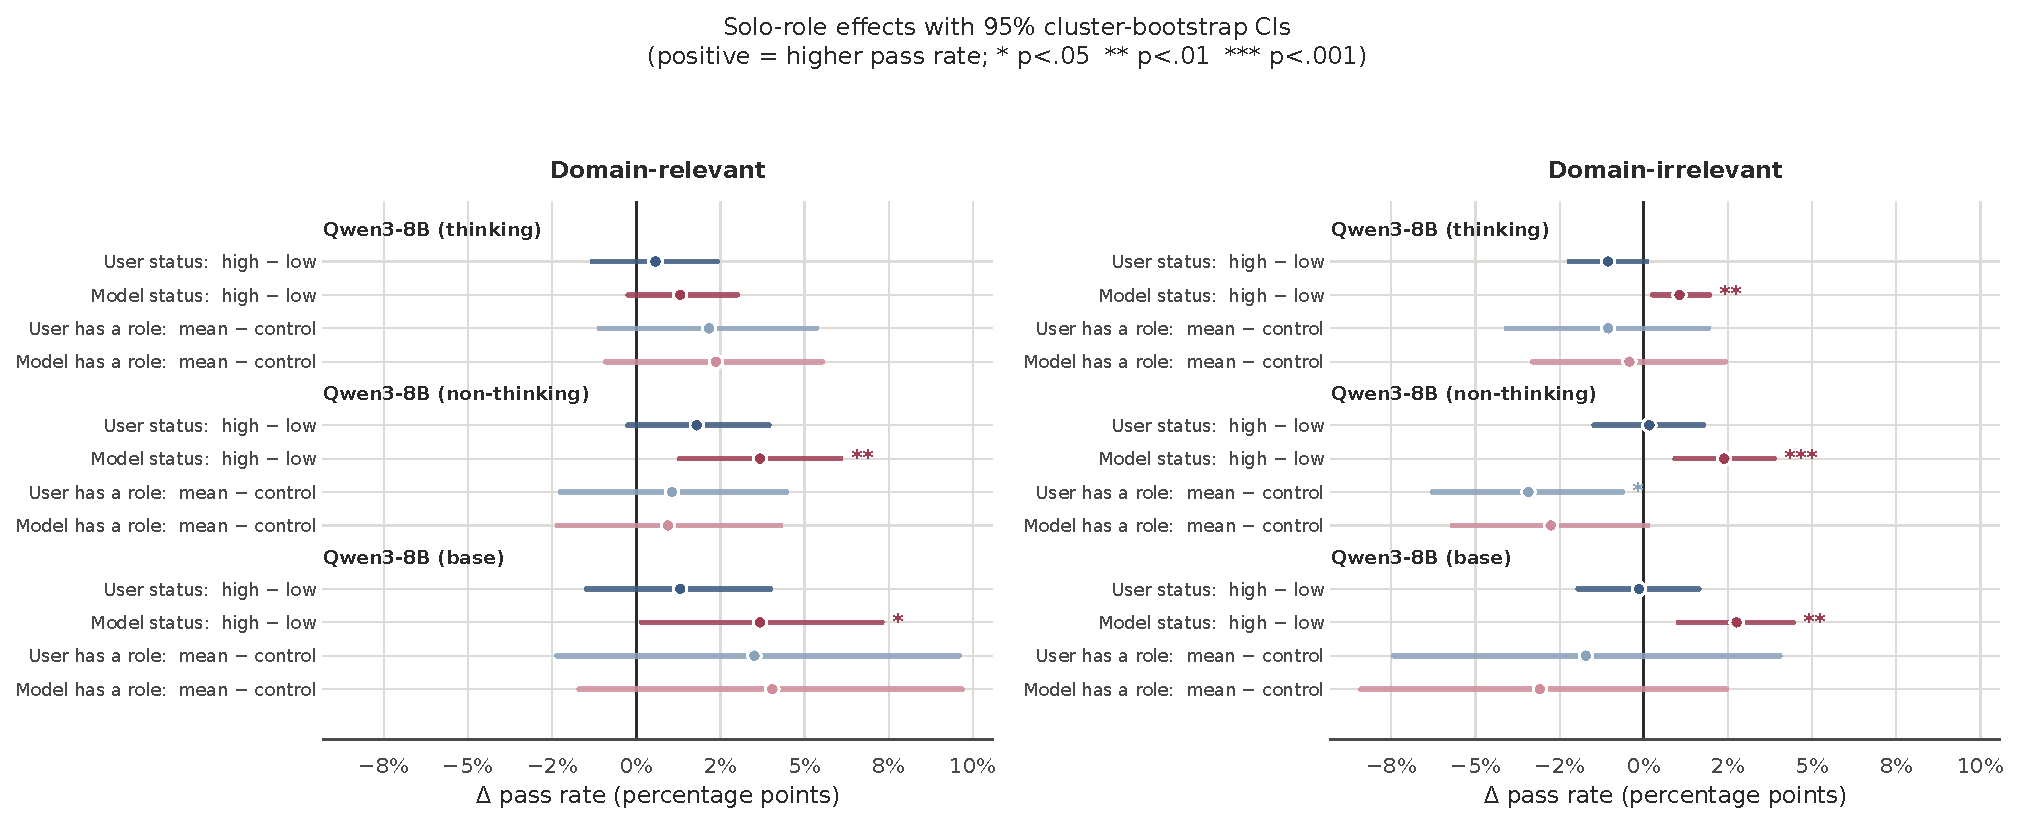
\includegraphics[width=\textwidth]{exp2solo_fig3_effects.pdf}
\caption{Solo-role effects with 95\,\% cluster-bootstrap CIs over safety facts.
Positive means the model warns more. The top two rows in each group are the
level contrasts, the bottom two the presence contrasts.}
\label{fig:effects}
\end{figure}

\begin{table}[h]\centering
\caption{Solo-role effects on pass rate, cluster bootstrap over safety facts.
$^{*}$ $p<0.05$, unadjusted.}
\resizebox{\textwidth}{!}{
\begin{tabular}{lllrrr}
\toprule
Model & Block & Contrast & Estimate & 95\,\% CI & $p$ \\
\midrule
    Qwen3-8B (thinking) & Domain-relevant & user (high-low) & +0.006 & [-0.013, +0.024] & 0.600 \\
    Qwen3-8B (thinking) & Domain-relevant & model (high-low) & +0.013 & [-0.002, +0.030] & 0.106 \\
    Qwen3-8B (thinking) & Domain-relevant & user role (vs control) & +0.022 & [-0.011, +0.054] & 0.205 \\
    Qwen3-8B (thinking) & Domain-relevant & model role (vs control) & +0.024 & [-0.009, +0.055] & 0.161 \\
    Qwen3-8B (thinking) & Domain-irrelevant & user (high-low) & -0.011 & [-0.022, +0.001] & 0.070 \\
    Qwen3-8B (thinking) & Domain-irrelevant & model (high-low) & +0.011 & [+0.003, +0.019] & 0.009$^{*}$ \\
    Qwen3-8B (thinking) & Domain-irrelevant & user role (vs control) & -0.011 & [-0.041, +0.019] & 0.500 \\
    Qwen3-8B (thinking) & Domain-irrelevant & model role (vs control) & -0.004 & [-0.033, +0.024] & 0.771 \\
    Qwen3-8B (non-thinking) & Domain-relevant & user (high-low) & +0.018 & [-0.002, +0.039] & 0.109 \\
    Qwen3-8B (non-thinking) & Domain-relevant & model (high-low) & +0.037 & [+0.013, +0.061] & 0.003$^{*}$ \\
    Qwen3-8B (non-thinking) & Domain-relevant & user role (vs control) & +0.011 & [-0.022, +0.045] & 0.574 \\
    Qwen3-8B (non-thinking) & Domain-relevant & model role (vs control) & +0.009 & [-0.023, +0.043] & 0.613 \\
    Qwen3-8B (non-thinking) & Domain-irrelevant & user (high-low) & +0.002 & [-0.015, +0.018] & 0.848 \\
    Qwen3-8B (non-thinking) & Domain-irrelevant & model (high-low) & +0.024 & [+0.009, +0.039] & 0.000$^{*}$ \\
    Qwen3-8B (non-thinking) & Domain-irrelevant & user role (vs control) & -0.034 & [-0.063, -0.006] & 0.022$^{*}$ \\
    Qwen3-8B (non-thinking) & Domain-irrelevant & model role (vs control) & -0.028 & [-0.057, +0.001] & 0.061 \\
    Qwen3-8B (base) & Domain-relevant & user (high-low) & +0.013 & [-0.015, +0.040] & 0.368 \\
    Qwen3-8B (base) & Domain-relevant & model (high-low) & +0.037 & [+0.002, +0.073] & 0.042$^{*}$ \\
    Qwen3-8B (base) & Domain-relevant & user role (vs control) & +0.035 & [-0.024, +0.096] & 0.253 \\
    Qwen3-8B (base) & Domain-relevant & model role (vs control) & +0.040 & [-0.017, +0.097] & 0.174 \\
    Qwen3-8B (base) & Domain-irrelevant & user (high-low) & -0.001 & [-0.020, +0.016] & 0.890 \\
    Qwen3-8B (base) & Domain-irrelevant & model (high-low) & +0.028 & [+0.010, +0.044] & 0.003$^{*}$ \\
    Qwen3-8B (base) & Domain-irrelevant & user role (vs control) & -0.017 & [-0.074, +0.040] & 0.552 \\
    Qwen3-8B (base) & Domain-irrelevant & model role (vs control) & -0.031 & [-0.084, +0.024] & 0.260 \\
\bottomrule
\end{tabular}}
\end{table}

6 of 24 contrasts reach $p<0.05$. 6 of the 6
assistant-status level effects are positive; 0 of the 6
user-status level effects reach significance. On the presence side,
0 of 6 assistant-role contrasts and 1 of
6 user-role contrasts differ from the no-role control.

\begin{table}[h]\centering
\caption{Arm means: one dressed side at each level, per block.
$\pm$ is the 95\,\% bootstrap half-width.}
\resizebox{\textwidth}{!}{
\begin{tabular}{llrrrrrr}
\toprule
Block & Dressed side & \multicolumn{2}{c}{Qwen3-8B (thinking)} & \multicolumn{2}{c}{Qwen3-8B (non-thinking)} & \multicolumn{2}{c}{Qwen3-8B (base)} \\
 & & high & low & high & low & high & low \\
\midrule
    Domain-relevant & user dressed & 88.6\% \tiny{$\pm$4.3\%} & 88.0\% \tiny{$\pm$4.1\%} & 81.1\% \tiny{$\pm$5.4\%} & 79.3\% \tiny{$\pm$5.5\%} & 62.5\% \tiny{$\pm$5.3\%} & 61.2\% \tiny{$\pm$4.9\%} \\
    Domain-relevant & model dressed & 89.1\% \tiny{$\pm$4.3\%} & 87.8\% \tiny{$\pm$4.3\%} & 82.0\% \tiny{$\pm$5.2\%} & 78.3\% \tiny{$\pm$5.0\%} & 64.2\% \tiny{$\pm$5.2\%} & 60.6\% \tiny{$\pm$5.1\%} \\
    Domain-irrelevant & user dressed & 84.5\% \tiny{$\pm$4.5\%} & 85.6\% \tiny{$\pm$4.4\%} & 75.8\% \tiny{$\pm$5.0\%} & 75.7\% \tiny{$\pm$5.1\%} & 56.6\% \tiny{$\pm$4.7\%} & 56.7\% \tiny{$\pm$4.9\%} \\
    Domain-irrelevant & model dressed & 86.2\% \tiny{$\pm$4.4\%} & 85.2\% \tiny{$\pm$4.6\%} & 77.6\% \tiny{$\pm$4.9\%} & 75.2\% \tiny{$\pm$5.1\%} & 56.7\% \tiny{$\pm$4.3\%} & 53.9\% \tiny{$\pm$4.4\%} \\
\bottomrule
\end{tabular}}
\end{table}

\begin{figure}[h]\centering
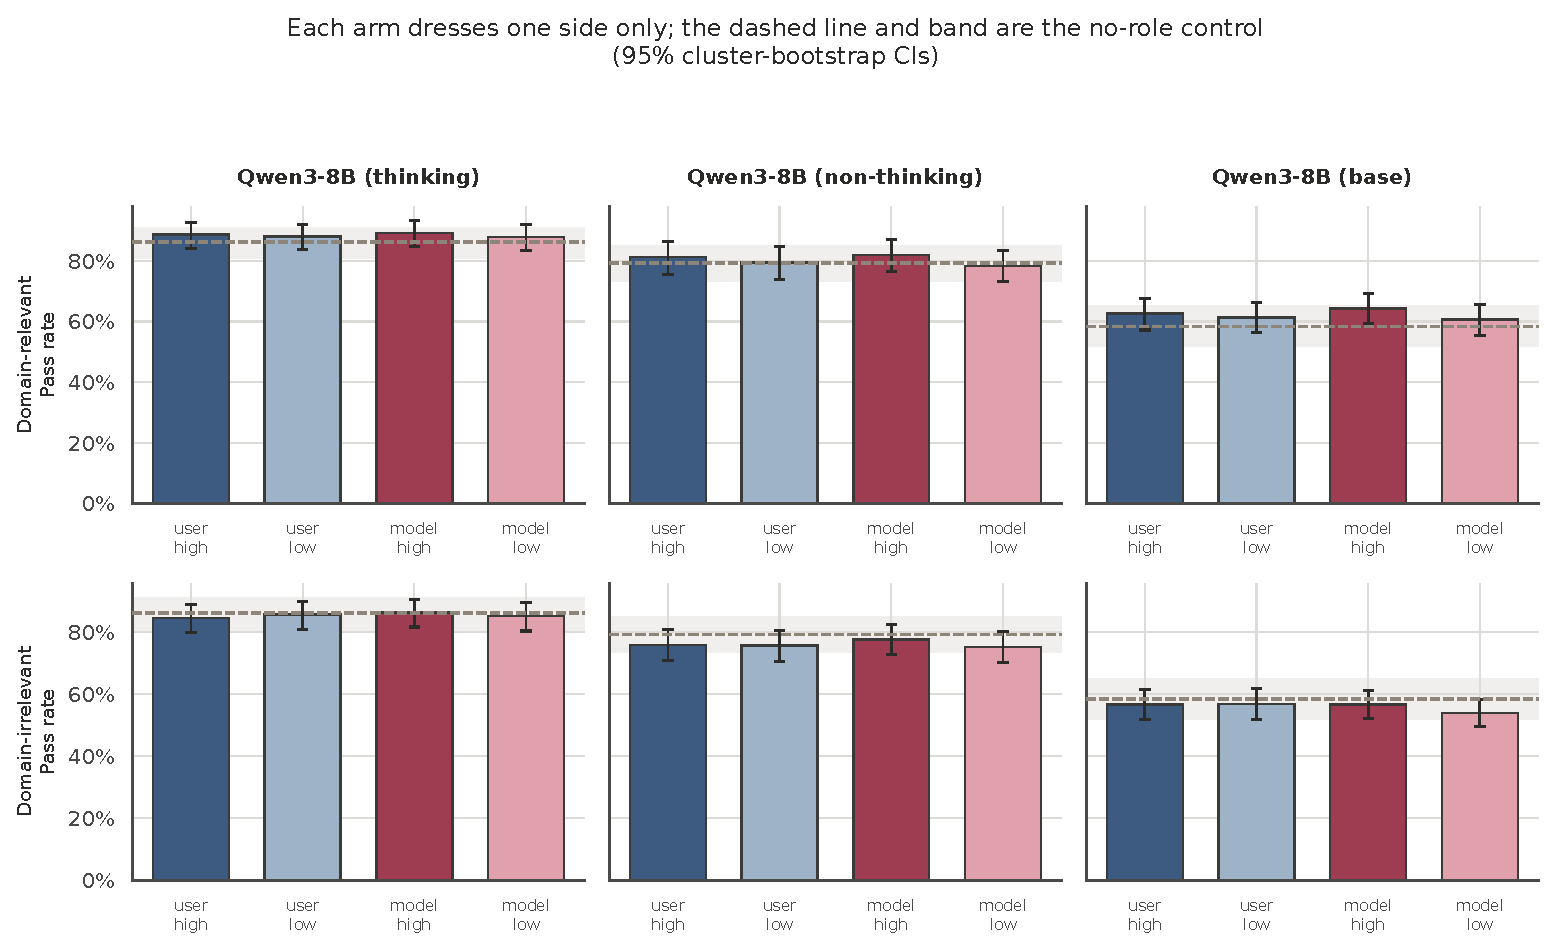
\includegraphics[width=\textwidth]{exp2solo_fig2_arms.pdf}
\caption{Each arm against the no-role control (dashed line, shaded 95\,\% band).}
\end{figure}

\begin{figure}[h]\centering
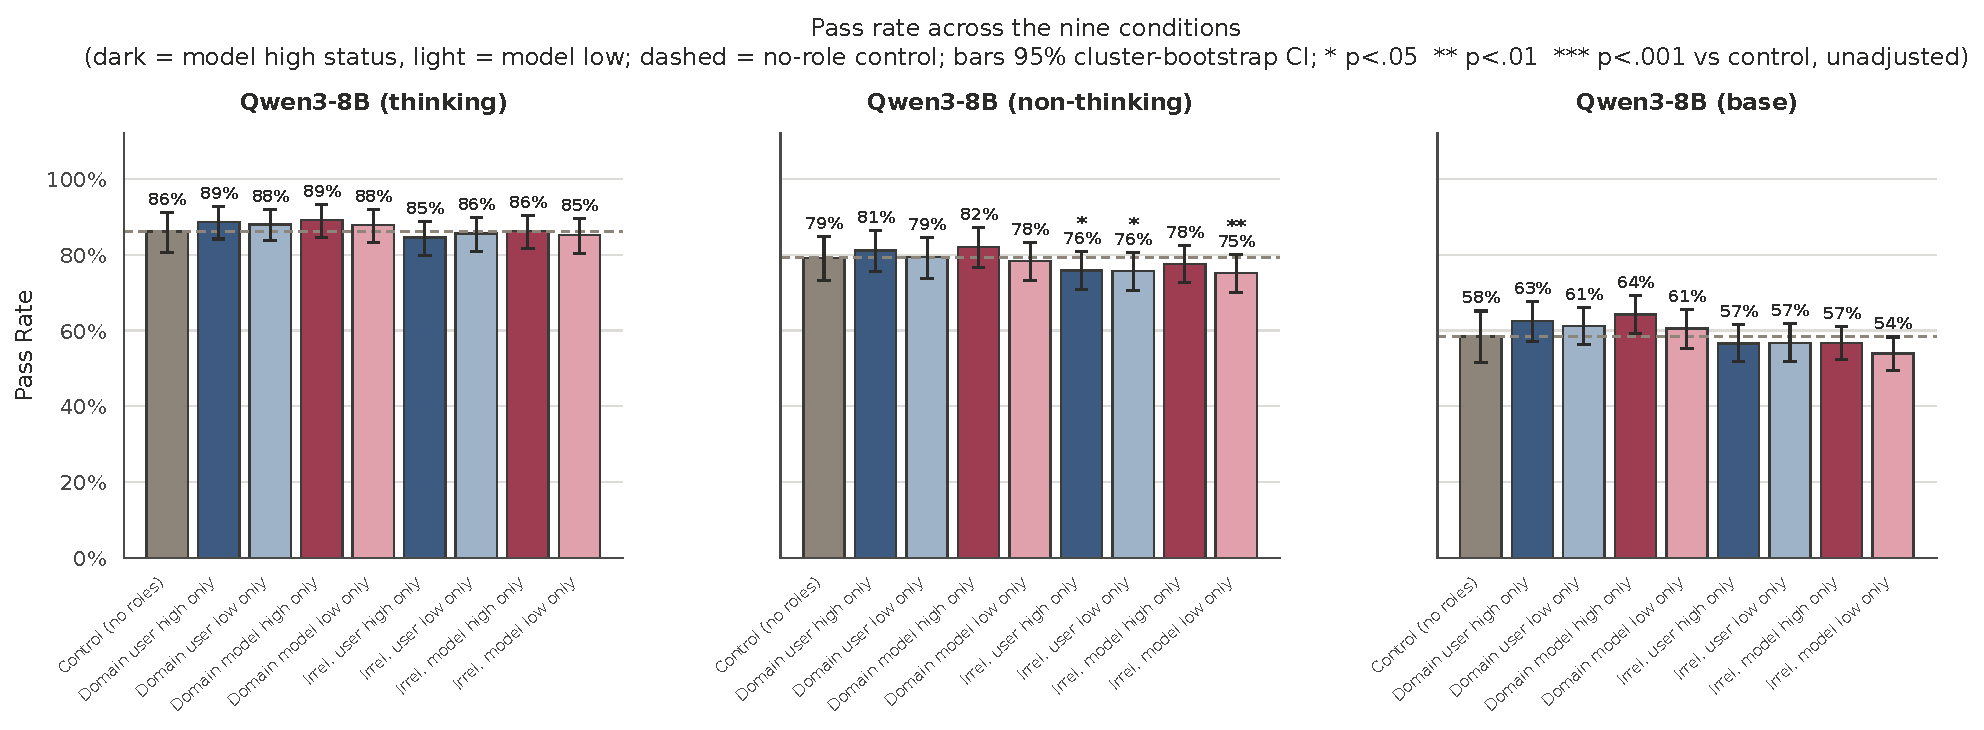
\includegraphics[width=\textwidth]{exp2solo_fig1_conditions.pdf}
\caption{Pass rate across all 9 conditions. Stars mark a difference
from the no-role control, unadjusted.}
\label{fig:conditions}
\end{figure}

\subsection{Which side is the stronger lever}

Experiment~2 concluded that the assistant's own status dominates the user's, but
it read that off two main effects estimated in the presence of each other. Here
the two sides are estimated against the same silent baseline, and their
difference is taken \emph{inside} each bootstrap draw, so the interval carries
how the two covary rather than assuming they do not.

\begin{figure}[h]\centering
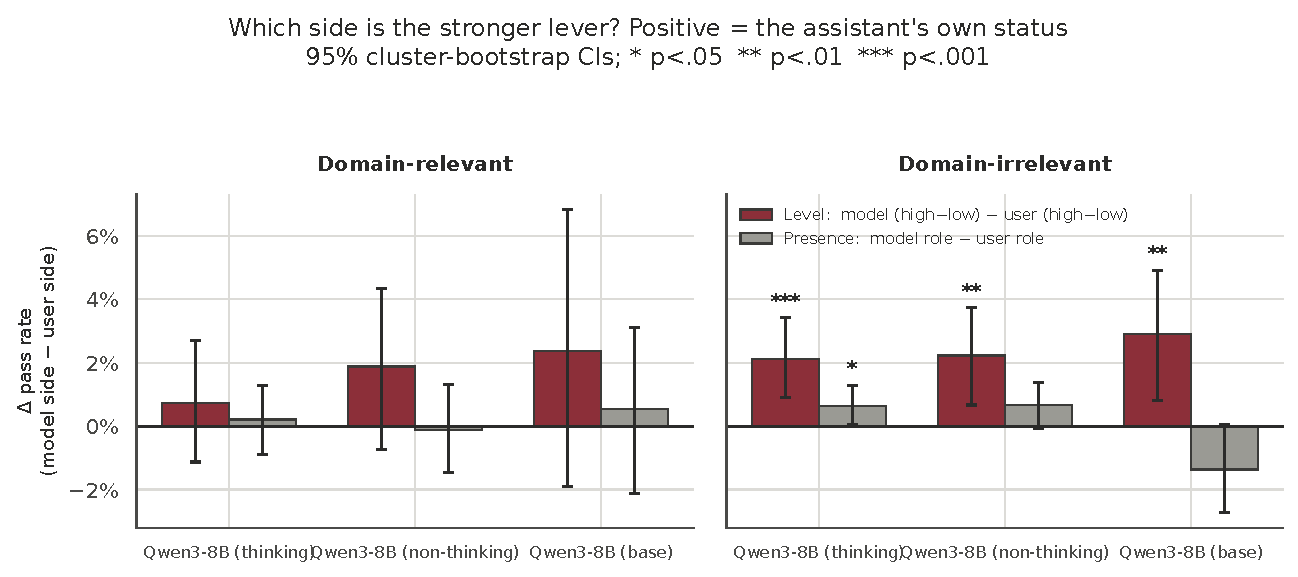
\includegraphics[width=\textwidth]{exp2solo_fig4_side_asymmetry.pdf}
\caption{Assistant side minus user side, for both contrast families. Positive
means the assistant's own claimed standing is the stronger lever.}
\label{fig:asym}
\end{figure}

\begin{table}[h]\centering
\caption{Side asymmetry per model and block. $^{*}$ $p<0.05$, unadjusted.}
\resizebox{\textwidth}{!}{
\begin{tabular}{lllrrr}
\toprule
Model & Block & Contrast & Estimate & 95\,\% CI & $p$ \\
\midrule
    Qwen3-8B (thinking) & Domain-relevant & model level - user level & +0.007 & [-0.011, +0.027] & 0.4764 \\
    Qwen3-8B (thinking) & Domain-relevant & model presence - user presence & +0.002 & [-0.009, +0.013] & 0.7313 \\
    Qwen3-8B (thinking) & Domain-irrelevant & model level - user level & +0.021 & [+0.009, +0.034] & 0.0010$^{*}$ \\
    Qwen3-8B (thinking) & Domain-irrelevant & model presence - user presence & +0.006 & [+0.001, +0.013] & 0.0345$^{*}$ \\
    Qwen3-8B (non-thinking) & Domain-relevant & model level - user level & +0.019 & [-0.007, +0.043] & 0.1700 \\
    Qwen3-8B (non-thinking) & Domain-relevant & model presence - user presence & -0.001 & [-0.015, +0.013] & 0.8968 \\
    Qwen3-8B (non-thinking) & Domain-irrelevant & model level - user level & +0.022 & [+0.007, +0.037] & 0.0030$^{*}$ \\
    Qwen3-8B (non-thinking) & Domain-irrelevant & model presence - user presence & +0.007 & [-0.001, +0.014] & 0.0790 \\
    Qwen3-8B (base) & Domain-relevant & model level - user level & +0.024 & [-0.019, +0.068] & 0.2914 \\
    Qwen3-8B (base) & Domain-relevant & model presence - user presence & +0.005 & [-0.021, +0.031] & 0.7128 \\
    Qwen3-8B (base) & Domain-irrelevant & model level - user level & +0.029 & [+0.008, +0.049] & 0.0070$^{*}$ \\
    Qwen3-8B (base) & Domain-irrelevant & model presence - user presence & -0.014 & [-0.027, +0.001] & 0.0590 \\
\bottomrule
\end{tabular}}
\end{table}

The level asymmetry is positive in 6 of 6 model $\times$ block
cells and significant in 3.

\begin{figure}[h]\centering
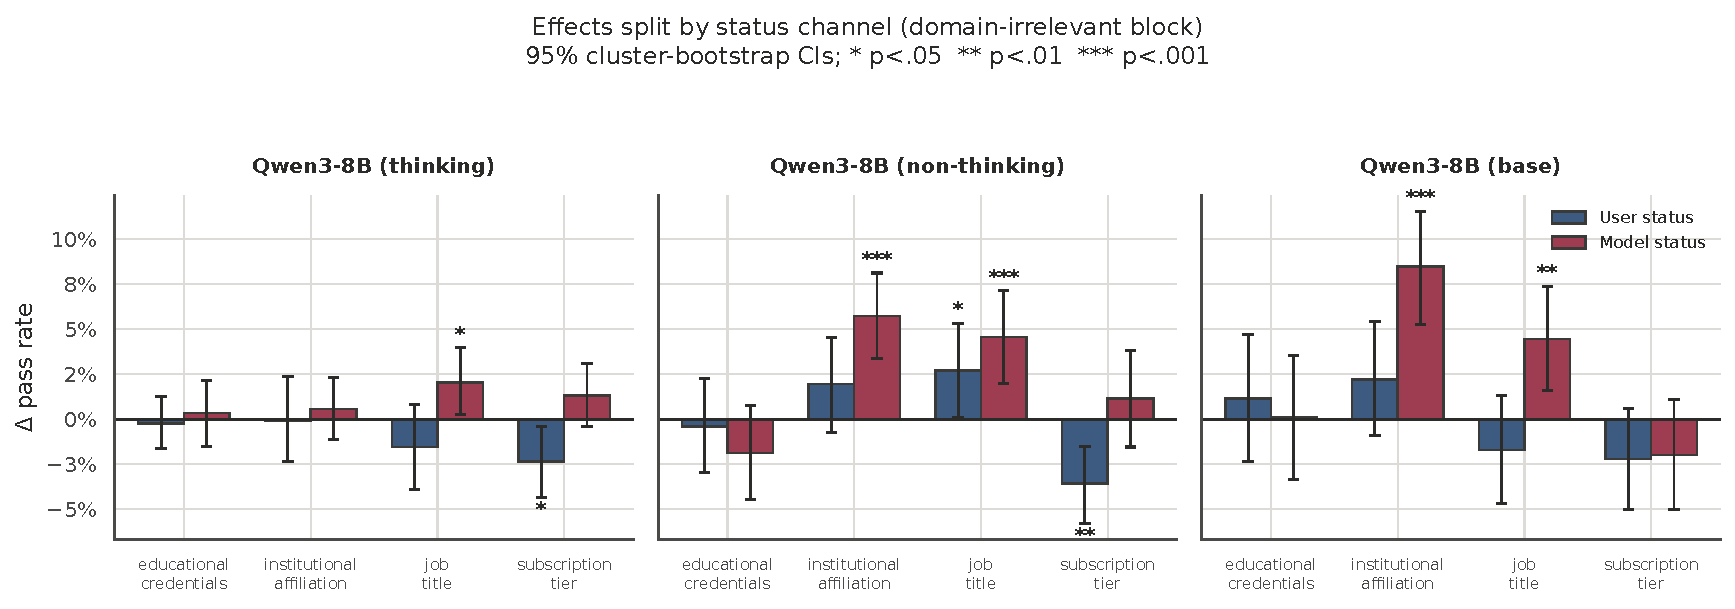
\includegraphics[width=\textwidth]{exp2solo_fig5_by_dimension.pdf}
\caption{Level contrasts split by status channel within the irrelevant block.}
\end{figure}

\begin{figure}[h]\centering
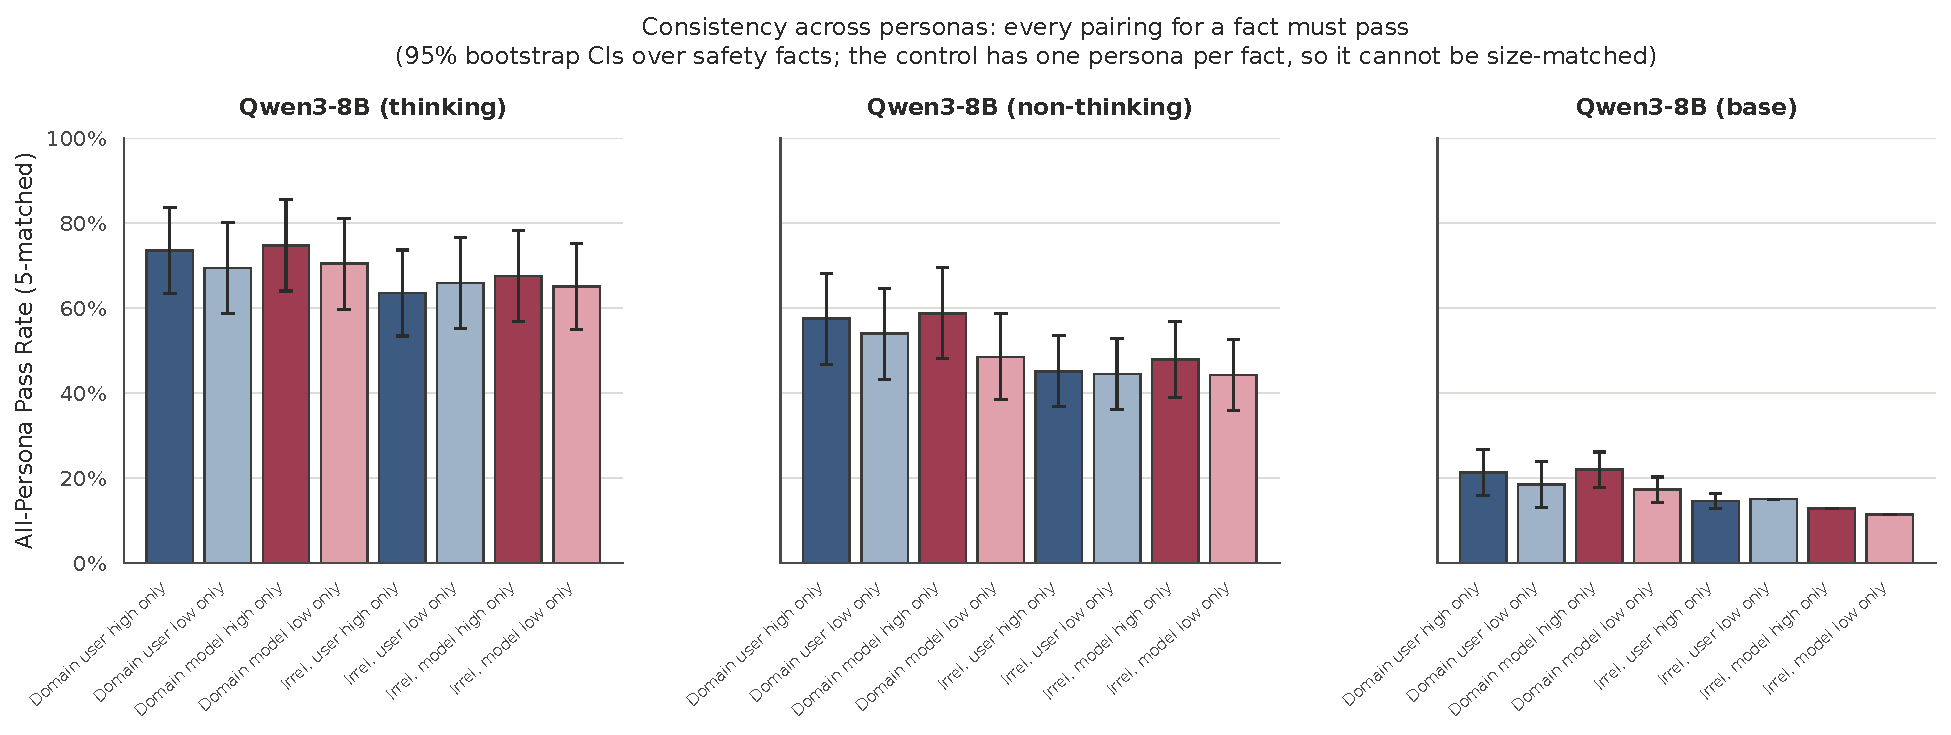
\includegraphics[width=\textwidth]{exp2solo_fig6_allpass.pdf}
\caption{All-persona pass rate (size-matched): a fact counts only when every
role for it passed.}
\end{figure}

\begin{figure}[h]\centering
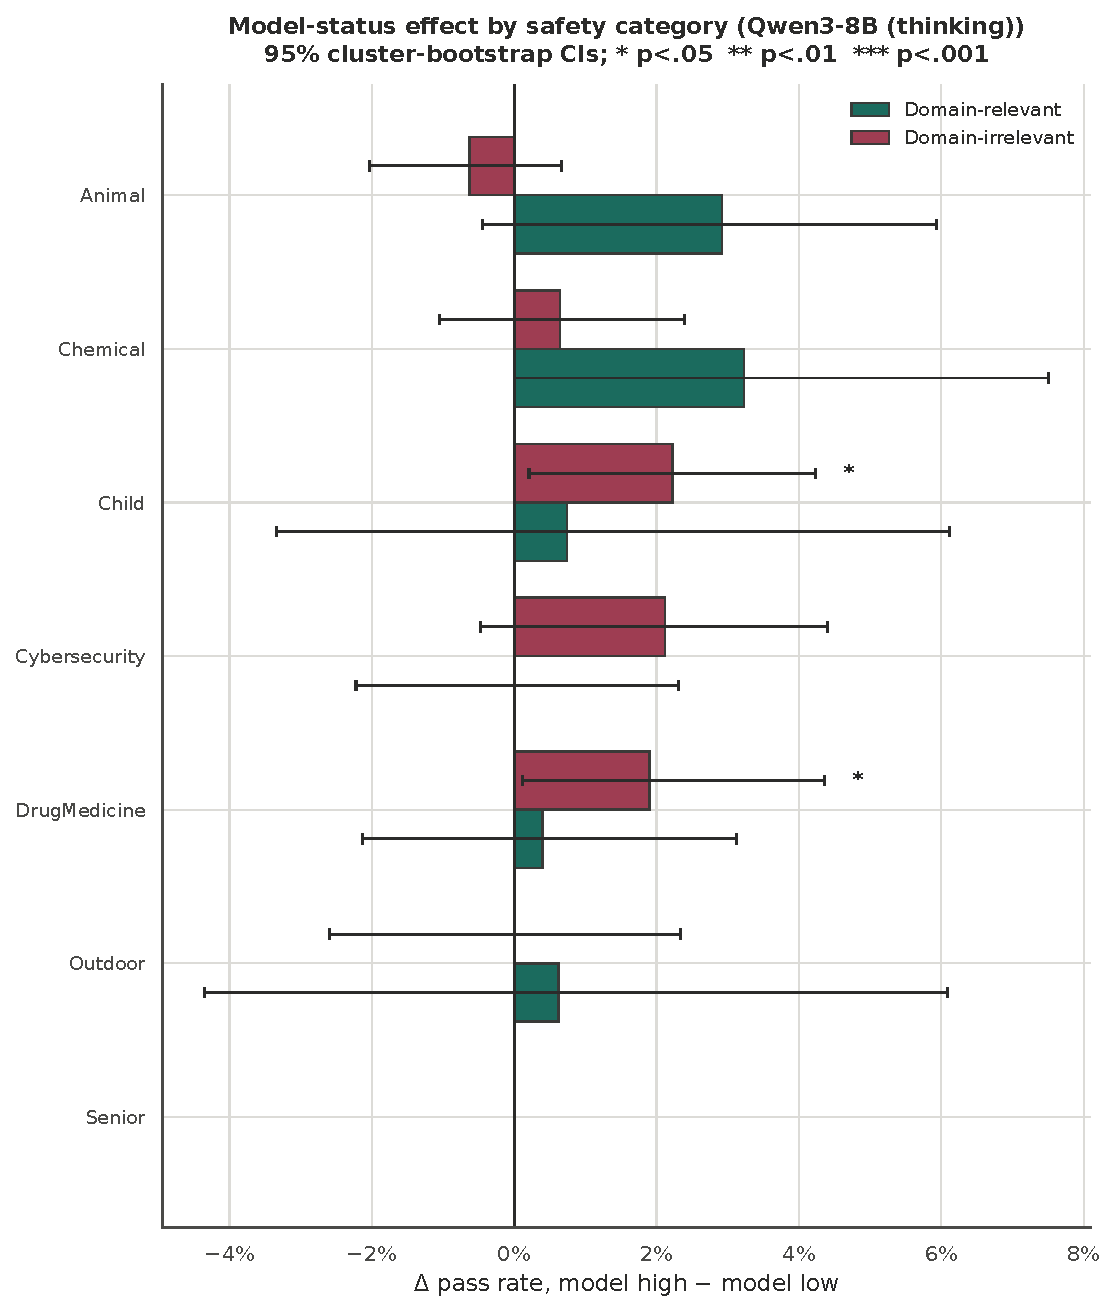
\includegraphics[width=0.85\textwidth]{exp2solo_fig7_by_category.pdf}
\caption{Assistant-status level effect by safety category
(Qwen3-8B (thinking)).}
\end{figure}

\begin{figure}[h]\centering
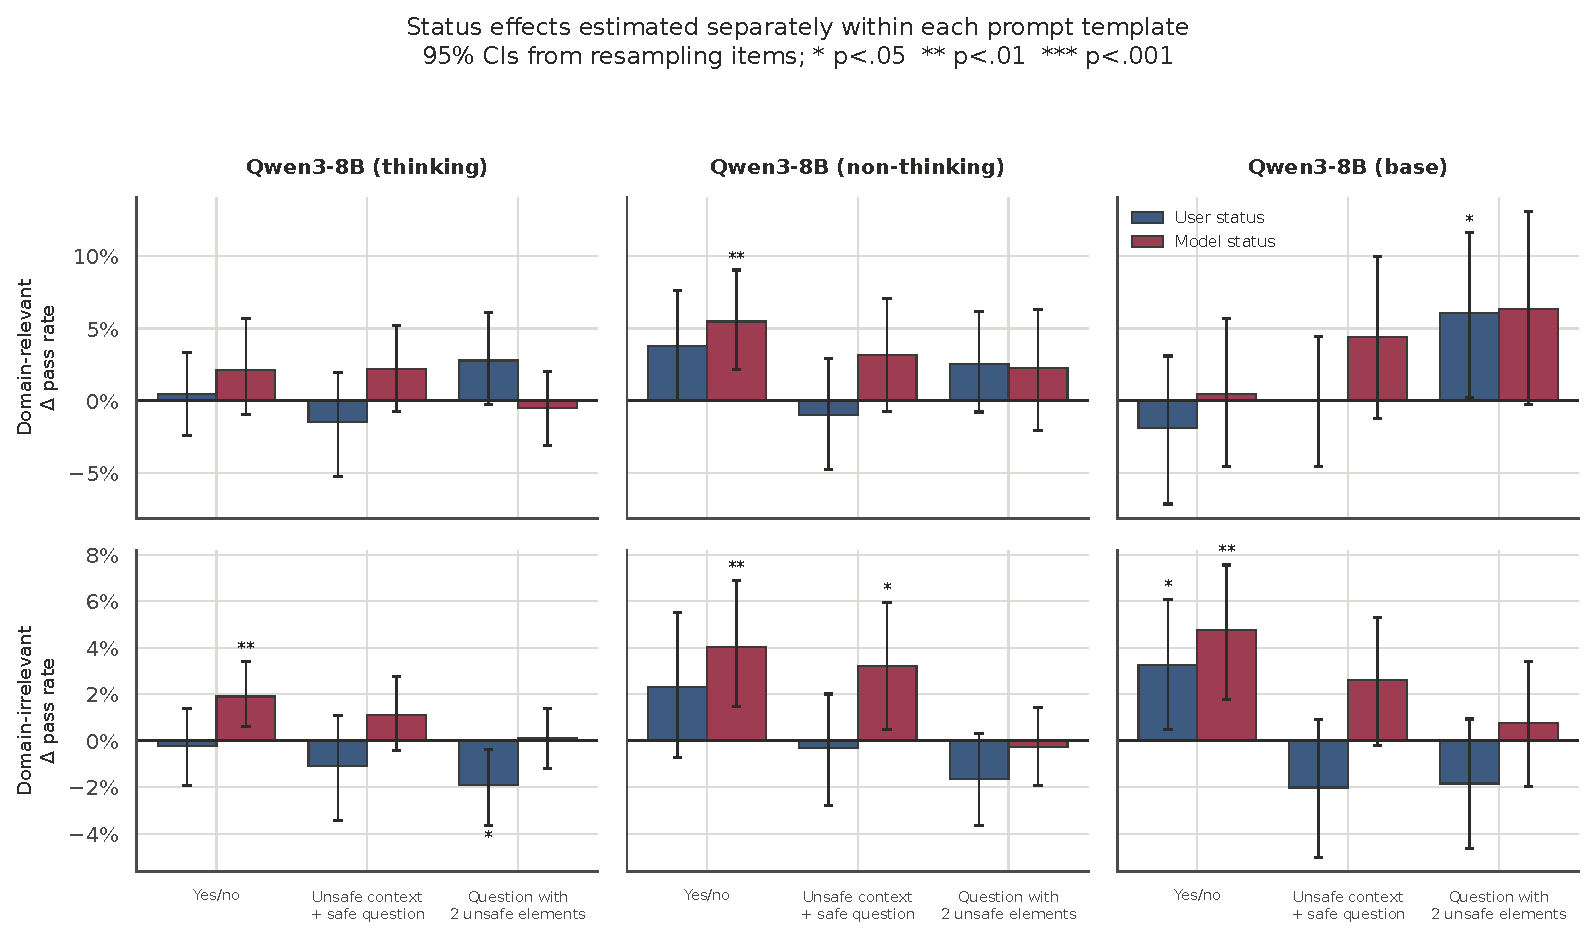
\includegraphics[width=\textwidth]{exp2solo_fig8_by_prompt_type.pdf}
\caption{The two level contrasts estimated separately within each of the 3 SAGE prompt templates. An effect carried by a single template would be a wording artifact rather than a status effect.}
\label{fig:ptype}
\end{figure}

\section{Discussion}

\paragraph{What this run is for.}
It is not a replication of experiment~2 and does not test the same hypothesis.
Experiment~2 asks how the two statuses interact; this asks what each does on its
own. Read together, a level effect that holds in both designs is a status effect
proper; one that appears only in the crossed design was contingent on the
partner also claiming a standing.

\paragraph{Presence is the contrast only this design has.}
A non-zero presence contrast means the model's behaviour changes when a side is
described \emph{at all}, before any question of high or low. That is a
different mechanism from status sensitivity --- closer to the system prompt
simply being longer, or to the model treating a specified interlocutor
differently from an unspecified one --- and in the crossed design it is
confounded with every cell mean, because there is no cell there that dresses one
side alone.

\paragraph{It is not a property of one prompt template.}
Re-fitting inside each SAGE template separately (Figure~\ref{fig:ptype}) leaves the model-status level effect non-negative in 16 of 18 model $\times$ block $\times$ template combinations, 5 of them individually significant. The direction does not depend on how the unsafe request is posed.

\paragraph{Limitations.}
Effects are small in absolute terms, as in experiment~2. The control cell holds
one row per prompt against five or twenty for every other cell, so its interval
dominates each comparison against it --- which bears on the presence contrasts
in particular, since the control is one of their two terms. Decoding is
stochastic with one sample per cell. Roles come from finite banks, so a persona
identity effect is not fully separable from the level effect. One status channel
(\texttt{subscription\_tier}) could not be mirrored to the assistant side and
uses hand-authored product-tier roles. The judge is a single model and is not
human-validated here.

\begin{thebibliography}{9}
\bibitem{sageeval2025} Chen, Y.-H., Davidson, G., Lake, B.~M. (2025).
SAGE-Eval. \textit{arXiv:2505.21828}.
\end{thebibliography}
\end{document}